\documentclass[11pt,a4paper]{article}
\usepackage[a4paper,margin=2.2cm,top=2cm,bottom=2.2cm]{geometry}
\usepackage[T1]{fontenc}
\usepackage[sc]{mathpazo}
\linespread{1.05}
\usepackage{amsmath,amssymb}
\usepackage{microtype}
\usepackage{booktabs}
\usepackage{graphicx}
\usepackage{xcolor}
\usepackage[font=small,labelfont=bf,skip=4pt]{caption}
\usepackage{enumitem}
\usepackage[hidelinks]{hyperref}
\usepackage{float}
\setlist{nosep,leftmargin=1.4em}
\setlength{\parskip}{0.35em}
\setlength{\parindent}{0pt}
\graphicspath{{../figures/}}
% Generated by scripts/run_analysis.py. Do not edit by hand.
% Use numeric macros inside math mode so minus signs render correctly.
\newcommand{\alphaA}{63}
\newcommand{\alphaB}{71}
\newcommand{\alphaC}{67}
\newcommand{\betaA}{39}
\newcommand{\betaB}{31}
\newcommand{\betaC}{35}
\newcommand{\crihiA}{0.709}
\newcommand{\crihiB}{0.781}
\newcommand{\crihiC}{0.745}
\newcommand{\criloA}{0.522}
\newcommand{\criloB}{0.604}
\newcommand{\criloC}{0.562}
\newcommand{\cseBA}{0.0668}
\newcommand{\cseBC}{0.0659}
\newcommand{\cseCA}{0.0678}
\newcommand{\cwaldhiBA}{0.211}
\newcommand{\cwaldhiBC}{0.169}
\newcommand{\cwaldhiCA}{0.173}
\newcommand{\cwaldloBA}{-0.051}
\newcommand{\cwaldloBC}{-0.089}
\newcommand{\cwaldloCA}{-0.093}
\newcommand{\dhiBA}{0.207}
\newcommand{\dhiBC}{0.167}
\newcommand{\dhiCA}{0.170}
\newcommand{\dloBA}{-0.051}
\newcommand{\dloBC}{-0.089}
\newcommand{\dloCA}{-0.092}
\newcommand{\dmeanBA}{0.078}
\newcommand{\dmeanBC}{0.039}
\newcommand{\dmeanCA}{0.039}
\newcommand{\dsdBA}{0.066}
\newcommand{\dsdBC}{0.065}
\newcommand{\dsdCA}{0.067}
\newcommand{\elossA}{0.0913}
\newcommand{\elossB}{0.0128}
\newcommand{\elossC}{0.0521}
\newcommand{\elossptsA}{9.13}
\newcommand{\elossptsB}{1.28}
\newcommand{\elossptsC}{5.21}
\newcommand{\emax}{0.7089}
\newcommand{\mcdraws}{2{,}000{,}000}
\newcommand{\mcmaxabsz}{0.71}
\newcommand{\mcpbestB}{0.6807}
\newcommand{\mcpgtBA}{0.8823}
\newcommand{\mcseBA}{0.00023}
\newcommand{\mcsebestB}{0.00033}
\newcommand{\mcseed}{20261008}
\newcommand{\mczBA}{-0.71}
\newcommand{\mczbestB}{0.54}
\newcommand{\meanA}{0.6176}
\newcommand{\meanB}{0.6961}
\newcommand{\meanC}{0.6569}
\newcommand{\meanfracA}{\tfrac{63}{102}}
\newcommand{\meanfracB}{\tfrac{71}{102}}
\newcommand{\meanfracC}{\tfrac{67}{102}}
\newcommand{\medianA}{0.6184}
\newcommand{\medianB}{0.6974}
\newcommand{\medianC}{0.6579}
\newcommand{\mleA}{0.62}
\newcommand{\mleB}{0.70}
\newcommand{\mleC}{0.66}
\newcommand{\mmeanexA}{0.617647}
\newcommand{\mmeanexB}{0.696078}
\newcommand{\mmeanexC}{0.656863}
\newcommand{\mmeanliA}{0.617600}
\newcommand{\mmeanliB}{0.696000}
\newcommand{\mmeanliC}{0.656800}
\newcommand{\mmeanlierrA}{-4.7\times 10^{-5}}
\newcommand{\mmeanlierrB}{-7.8\times 10^{-5}}
\newcommand{\mmeanlierrC}{-6.3\times 10^{-5}}
\newcommand{\mmeantkA}{0.617595}
\newcommand{\mmeantkB}{0.696016}
\newcommand{\mmeantkC}{0.656805}
\newcommand{\mmeantkerrA}{-5.2\times 10^{-5}}
\newcommand{\mmeantkerrB}{-6.2\times 10^{-5}}
\newcommand{\mmeantkerrC}{-5.7\times 10^{-5}}
\newcommand{\moddsexA}{1.657895}
\newcommand{\moddsexB}{2.366667}
\newcommand{\moddsexC}{1.970588}
\newcommand{\moddsliA}{1.657895}
\newcommand{\moddsliB}{2.366667}
\newcommand{\moddsliC}{1.970588}
\newcommand{\moddslierrA}{0}
\newcommand{\moddslierrB}{0}
\newcommand{\moddslierrC}{0}
\newcommand{\moddstkA}{1.657832}
\newcommand{\moddstkB}{2.366480}
\newcommand{\moddstkC}{1.970479}
\newcommand{\moddstkerrA}{-6.3\times 10^{-5}}
\newcommand{\moddstkerrB}{-1.9\times 10^{-4}}
\newcommand{\moddstkerrC}{-1.1\times 10^{-4}}
\newcommand{\modeA}{0.6200}
\newcommand{\modeB}{0.7000}
\newcommand{\modeC}{0.6600}
\newcommand{\onempBA}{0.884}
\newcommand{\onempBC}{0.728}
\newcommand{\onempCA}{0.722}
\newcommand{\pbestA}{0.071}
\newcommand{\pbestB}{0.681}
\newcommand{\pbestC}{0.248}
\newcommand{\pbestlongA}{0.071201793908}
\newcommand{\pbestlongB}{0.680515173383}
\newcommand{\pbestlongC}{0.248283032709}
\newcommand{\pgtBA}{0.882}
\newcommand{\pgtBC}{0.726}
\newcommand{\pgtCA}{0.721}
\newcommand{\pgtlongBA}{0.882419268177}
\newcommand{\pgtlongBC}{0.726473157011}
\newcommand{\pgtlongCA}{0.720933436473}
\newcommand{\pmarginBA}{0.667}
\newcommand{\pmarginBC}{0.435}
\newcommand{\pmarginCA}{0.437}
\newcommand{\predcovA}{0.961}
\newcommand{\predcovB}{0.965}
\newcommand{\predcovC}{0.958}
\newcommand{\predhiA}{75}
\newcommand{\predhiB}{82}
\newcommand{\predhiC}{78}
\newcommand{\predloA}{48}
\newcommand{\predloB}{56}
\newcommand{\predloC}{52}
\newcommand{\predmeanA}{61.8}
\newcommand{\predmeanB}{69.6}
\newcommand{\predmeanC}{65.7}
\newcommand{\predsdA}{6.8}
\newcommand{\predsdB}{6.4}
\newcommand{\predsdC}{6.6}
\newcommand{\pvalBA}{0.116}
\newcommand{\pvalBC}{0.272}
\newcommand{\pvalCA}{0.278}
\newcommand{\sBtendec}{B}
\newcommand{\sBtenelossB}{0.0135}
\newcommand{\sBtenmeanB}{0.667}
\newcommand{\sBtenpBA}{0.859}
\newcommand{\sBtenpBC}{0.707}
\newcommand{\sBtenpbestA}{0.086}
\newcommand{\sBtenpbestB}{0.652}
\newcommand{\sBtenpbestC}{0.262}
\newcommand{\sBttdec}{B}
\newcommand{\sBttelossB}{0.0129}
\newcommand{\sBttmeanB}{0.692}
\newcommand{\sBttpBA}{0.880}
\newcommand{\sBttpBC}{0.724}
\newcommand{\sBttpbestA}{0.073}
\newcommand{\sBttpbestB}{0.677}
\newcommand{\sBttpbestC}{0.250}
\newcommand{\sJefdec}{B}
\newcommand{\sJefelossB}{0.0128}
\newcommand{\sJefmeanB}{0.698}
\newcommand{\sJefpBA}{0.884}
\newcommand{\sJefpBC}{0.728}
\newcommand{\sJefpbestA}{0.070}
\newcommand{\sJefpbestB}{0.682}
\newcommand{\sJefpbestC}{0.247}
\newcommand{\sUnidec}{B}
\newcommand{\sUnielossB}{0.0128}
\newcommand{\sUnimeanB}{0.696}
\newcommand{\sUnipBA}{0.882}
\newcommand{\sUnipBC}{0.726}
\newcommand{\sUnipbestA}{0.071}
\newcommand{\sUnipbestB}{0.681}
\newcommand{\sUnipbestC}{0.248}
\newcommand{\scenapBA}{0.882}
\newcommand{\scenapBC}{0.726}
\newcommand{\scenapbest}{0.681}
\newcommand{\scenbpBA}{0.954}
\newcommand{\scenbpBC}{0.804}
\newcommand{\scenbpbest}{0.785}
\newcommand{\scencpBA}{0.981}
\newcommand{\scencpBC}{0.853}
\newcommand{\scencpbest}{0.845}
\newcommand{\scencross}{750}
\newcommand{\scendpBA}{0.996}
\newcommand{\scendpBC}{0.912}
\newcommand{\scendpbest}{0.911}
\newcommand{\scenepBA}{{>}\,0.999}
\newcommand{\scenepBC}{0.972}
\newcommand{\scenepbest}{0.972}
\newcommand{\sdA}{0.0479}
\newcommand{\sdB}{0.0453}
\newcommand{\sdC}{0.0468}
\newcommand{\shrinkw}{0.980}
\newcommand{\waldhiA}{0.715}
\newcommand{\waldhiB}{0.790}
\newcommand{\waldhiC}{0.753}
\newcommand{\waldloA}{0.525}
\newcommand{\waldloB}{0.610}
\newcommand{\waldloC}{0.567}
\newcommand{\waldseA}{0.0485}
\newcommand{\waldseB}{0.0458}
\newcommand{\waldseC}{0.0474}
\newcommand{\zpoolBA}{1.19}
\newcommand{\zpoolBC}{0.61}
\newcommand{\zpoolCA}{0.59}

% Group members. The report's title block and its PDF metadata both read this file.
\newcommand{\projectauthors}{%
  Aditya Singh (250003007) \quad Hiransh Anand (250041018) \quad Parth Pawar (250041030)\\
  Tirthanker Singh (250003081) \quad Gulam Abbas (250041016)}
\newcommand{\projectauthorsplain}{Aditya Singh, Hiransh Anand, Parth Pawar, Tirthanker Singh, Gulam Abbas}

\hypersetup{pdftitle={Which Treatment Should We Choose? A Bayesian comparison of three treatments},
  pdfauthor={\projectauthorsplain}, pdfsubject={MA 232 Bayesian Statistical Methods, Group Project 2}}

\newcommand{\Beta}{\mathrm{Beta}}
\newcommand{\tA}{\theta_A}
\newcommand{\tB}{\theta_B}
\newcommand{\tC}{\theta_C}
\newcommand{\course}[1]{\textcolor{black!60}{\small[#1]}}

\title{\vspace{-1.2em}\textbf{Which Treatment Should We Choose?}\\[0.3em]
\large A Bayesian comparison of three treatments}
\author{MA 232 Bayesian Statistical Methods \,·\, Group Project 2\\[0.2em]
\projectauthors}
\date{October 2026}

\begin{document}
\maketitle
\vspace{-1.5em}

\begin{center}
\fbox{\parbox{0.93\linewidth}{\small
\textbf{Summary.} With independent uniform priors, the posterior success probabilities are
$\tA\sim\Beta(\alphaA,\betaA)$, $\tB\sim\Beta(\alphaB,\betaB)$ and $\tC\sim\Beta(\alphaC,\betaC)$.
Treatment B has the highest posterior mean ($\meanB$). The posterior probability that B is better
than A is $\pgtBA$, and that B is the best of the three is $\pbestB$; both are computed exactly, not
simulated. Choosing B has the smallest expected loss, $\elossptsB$ percentage points of success rate,
and B is chosen under every prior we tried. We recommend \textbf{treatment B}, while noting that the
evidence that B beats C is weak (probability $\pgtBC$).}}
\end{center}

\section{Problem and data}

The project sheet gives simulated clinical-trial data for three treatments (Table~\ref{tab:data}).
It asks for: (1) the estimated success probabilities, (2) the differences between treatments,
(3) the uncertainty in the estimates, (4) the Bayesian posterior distributions, (5) the probability
that B is better than A, (6) the probability that B is the best treatment, and (7) a final
recommendation. Sections~3--6 answer these in order. Section~7 checks the Module~5
approximations against our exact answers.

\begin{table}[H]
\centering\small
\caption{Trial data (project sheet, Project~2).}\label{tab:data}
\begin{tabular}{lrrrc}
\toprule
Treatment & Patients $n$ & Successes $s$ & Failures $n-s$ & Sample proportion $s/n$\\
\midrule
A & 100 & 62 & 38 & $\mleA$\\
B & 100 & 70 & 30 & $\mleB$\\
C & 100 & 66 & 34 & $\mleC$\\
\bottomrule
\end{tabular}
\end{table}

\textbf{Assumptions.} Within a treatment, patients respond independently with a common success
probability $\theta_k$. The three groups contain different patients and are analysed independently.
Each outcome is a simple success or failure. Section~8 discusses these assumptions.

\section{Model}

\textbf{Likelihood and sufficiency.} For one treatment, let $x_1,\dots,x_n\in\{0,1\}$ be the
outcomes, with $s=\sum x_i$. Each $x_i\sim\mathrm{Bernoulli}(\theta)$, so
\[
f(\mathbf{x}\mid\theta)=\prod_{i=1}^{n}\theta^{x_i}(1-\theta)^{1-x_i}
=\underbrace{\theta^{s}(1-\theta)^{n-s}}_{g_\theta(s)}\cdot\underbrace{1}_{h(\mathbf{x})}.
\]
By the Neyman--Fisher factorisation, $s$ is sufficient for $\theta$
\course{Module~3, \S2, p.\,4}. Only the counts in Table~\ref{tab:data} matter, not the order in
which patients were treated. The likelihood is maximised at $\hat\theta_{\text{MLE}}=s/n$
\course{Module~3, p.\,14}.

\textbf{Prior and posterior.} With a $\Beta(\alpha,\beta)$ prior,
$\pi(\theta\mid\mathbf{x})\propto\theta^{s+\alpha-1}(1-\theta)^{n-s+\beta-1}$, so
\[
\theta\mid\mathbf{x}\sim\Beta(s+\alpha,\;n-s+\beta)
\qquad\text{\course{Module~4, Example~4.6, pp.\,4--5}.}
\]
Our main prior is the uniform $\Beta(1,1)$. It expresses no preference between success rates and
treats the three treatments identically. It gives
$\tA\mid\text{data}\sim\Beta(\alphaA,\betaA)$, $\tB\mid\text{data}\sim\Beta(\alphaB,\betaB)$ and
$\tC\mid\text{data}\sim\Beta(\alphaC,\betaC)$. Because the groups and priors are independent, the
joint posterior is the product of the three, which makes the joint probabilities in
Sections~4--5 computable. Section~6 repeats the key results under three other priors.

\textbf{Bayes estimators.} The point estimate depends on the loss function
\course{Module~4, Theorems~4.1--4.3, pp.\,7--8}. For a $\Beta(a,b)$ posterior:
\begin{itemize}
\item squared-error loss gives the posterior mean $a/(a+b)$;
\item absolute-error loss gives the posterior median, which has no closed form and is computed numerically;
\item zero--one loss gives the posterior mode $(a-1)/(a+b-2)$.
\end{itemize}

\section{Estimates, uncertainty and posterior distributions (questions 1, 3, 4)}

\begin{table}[H]
\centering\small
\caption{Point estimates and 95\% intervals. CrI: equal-tailed credible interval from the Beta
posterior. CI: classical Wald interval $\hat\theta\pm1.96\sqrt{\hat\theta(1-\hat\theta)/n}$.}\label{tab:est}
\begin{tabular}{lccccccc}
\toprule
 & MLE & Post.\ mean & Post.\ median & Post.\ mode & Post.\ sd & 95\% CrI & 95\% Wald CI\\
\midrule
A & $\mleA$ & $\meanA$ & $\medianA$ & $\modeA$ & $\sdA$ & $(\criloA,\ \crihiA)$ & $(\waldloA,\ \waldhiA)$\\
B & $\mleB$ & $\meanB$ & $\medianB$ & $\modeB$ & $\sdB$ & $(\criloB,\ \crihiB)$ & $(\waldloB,\ \waldhiB)$\\
C & $\mleC$ & $\meanC$ & $\medianC$ & $\modeC$ & $\sdC$ & $(\criloC,\ \crihiC)$ & $(\waldloC,\ \waldhiC)$\\
\bottomrule
\end{tabular}
\end{table}

\begin{figure}[H]
\centering
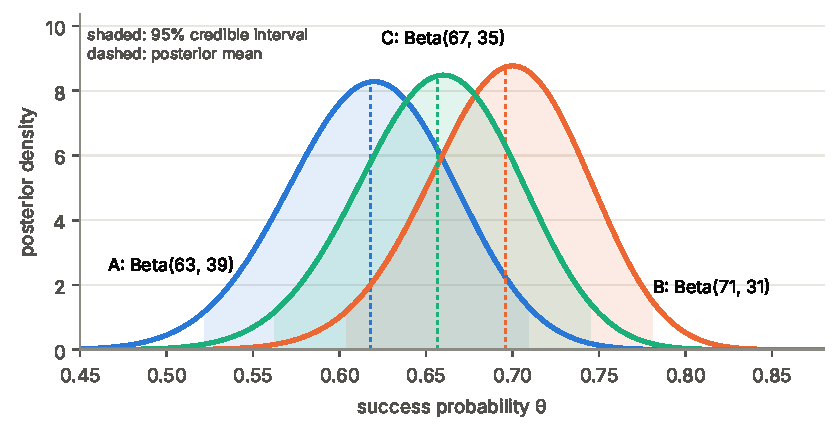
\includegraphics[width=0.86\linewidth]{fig1_posteriors.pdf}
\caption{Posterior densities of the three success probabilities under uniform priors. The curves
overlap substantially: B is ahead, but none of the three is clearly separated from the others.}
\label{fig:post}
\end{figure}

\textbf{Reading the estimates.} The posterior mean of B is $\meanfracB=\meanB$. As in every conjugate
model in the course, it is a weighted average of the MLE and the prior mean:
$\frac{s+1}{n+2}=\frac{n}{n+2}\cdot\frac{s}{n}+\frac{2}{n+2}\cdot\frac12$. With $n=100$, the data
weight is $\shrinkw$, so the prior moves each estimate only slightly towards $\tfrac12$. Under the
uniform prior the posterior mode equals the MLE. Each posterior has $\alpha>\beta$, so it is
left-skewed, and mean $<$ median $<$ mode, as Table~\ref{tab:est} shows
\course{the same ordering as Module~4, Example~4.9}.

\textbf{Uncertainty.} Each posterior standard deviation is about $0.045$--$0.048$, so each success
rate is known to within roughly $\pm9$ percentage points (95\%). The credible and Wald intervals
almost coincide numerically, but they mean different things. The credible interval is a probability
statement about $\theta$ given these data: $P(\criloB<\tB<\crihiB\mid\text{data})=0.95$. The Wald
interval describes a procedure that covers the true $\theta$ in 95\% of repeated trials.

\textbf{Predictions for future patients.} The probability that the next patient on a treatment
succeeds is that treatment's posterior mean. For 100 new patients on B, the number of successes
follows a beta--binomial distribution with mean $\predmeanB$ and standard deviation $\predsdB$.
Its 95\% predictive interval is $\predloB$--$\predhiB$ successes; on the integer scale this
actually covers $\predcovB$. Predictive intervals are wider than credible intervals, because they
add patient-to-patient variation to the uncertainty about $\tB$.

\section{\texorpdfstring{Differences between treatments, and $P(\tB>\tA)$ (questions 2 and 5)}{Differences between treatments, and P(B > A) (questions 2 and 5)}}

For a pair of treatments, the posterior of the difference, such as $\delta=\tB-\tA$, is the
distribution of a difference of independent Beta variables. Its mean is the difference of the
posterior means, its variance is the sum of the variances, and its quantiles come from
\[
P(\tB-\tA\le d\mid\text{data})=\int_0^1 f_B(t)\,\bigl[1-F_A(t-d)\bigr]\,dt .
\]
Here $f_k$ and $F_k$ are the posterior density and CDF of $\theta_k$.

\textbf{An exact answer for $P(\tB>\tA)$.} Setting $d=0$,
\[
P(\tB>\tA\mid\text{data})=\int_0^1 f_B(t)\,F_A(t)\,dt .
\]
Both Beta parameters are whole numbers, so $f_B$ and $F_A$ are polynomials in $t$ with rational
coefficients. For example, $F_A(t)=\sum_{j=63}^{101}\binom{101}{j}t^j(1-t)^{101-j}$, the binomial-tail
form of the Beta CDF. The integral is therefore an exact rational number, which we compute in
exact fraction arithmetic:
\[
P(\tB>\tA\mid\text{data})=\pgtlongBA\ldots
\]
We obtained the same fraction from an independent finite-sum formula. Numerical quadrature agrees
to $10^{-12}$. A Monte Carlo run with $\mcdraws$ posterior draws gives $\mcpgtBA$, which is
$\mczBA$ standard errors from the exact value.

\begin{table}[H]
\centering\small
\caption{Pairwise differences. Bayesian columns are posterior summaries; the last two columns
give the classical Wald interval and one-sided $z$-test of the same difference.}\label{tab:diff}
\begin{tabular}{lcccccc}
\toprule
Difference & Post.\ mean & 95\% CrI & $P(\delta>0)$ & $P(\delta>0.05)$ & 95\% Wald CI & One-sided $p$\\
\midrule
$\tB-\tA$ & $\dmeanBA$ & $(\dloBA,\ \dhiBA)$ & $\pgtBA$ & $\pmarginBA$ & $(\cwaldloBA,\ \cwaldhiBA)$ & $\pvalBA$\\
$\tB-\tC$ & $\dmeanBC$ & $(\dloBC,\ \dhiBC)$ & $\pgtBC$ & $\pmarginBC$ & $(\cwaldloBC,\ \cwaldhiBC)$ & $\pvalBC$\\
$\tC-\tA$ & $\dmeanCA$ & $(\dloCA,\ \dhiCA)$ & $\pgtCA$ & $\pmarginCA$ & $(\cwaldloCA,\ \cwaldhiCA)$ & $\pvalCA$\\
\bottomrule
\end{tabular}
\end{table}

\begin{figure}[H]
\centering
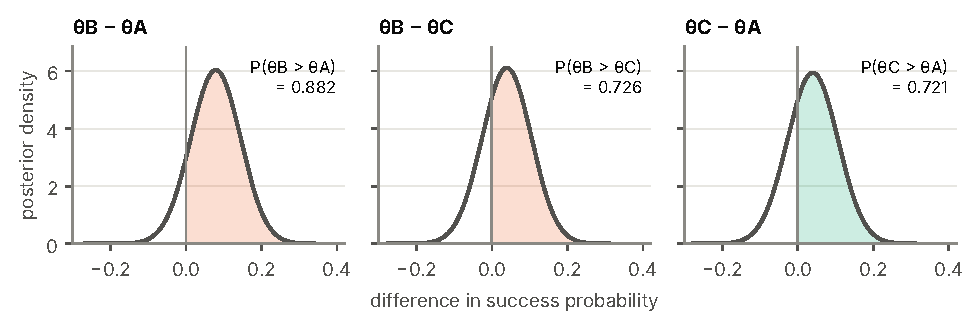
\includegraphics[width=0.9\linewidth]{fig2_differences.pdf}
\caption{Posterior densities of the pairwise differences. The shaded area to the right of zero is
the posterior probability that the first treatment is better.}
\label{fig:diff}
\end{figure}

\textbf{Reading the differences.} Every 95\% credible interval for a difference contains zero, so
no difference is settled at that level. The Bayesian answer to ``is B better than A?'' is still
direct: probability $\pgtBA$. The classical test of the same comparison gives $p=\pvalBA$, which is
``not significant'' at 5\% and says nothing about how likely B is to be better. Under flat priors and
large samples the two numbers are related, since $1-p=\onempBA\approx\pgtBA$, but only the posterior
probability answers the question the clinician asks. A difference may also be too small to matter.
The probability that B beats A by more than 5 percentage points is only $\pmarginBA$.

\section{Which treatment is best? (question 6)}

Treatment $k$ is best when $\theta_k$ exceeds both others. By independence,
\[
P(k\text{ is best}\mid\text{data})=\int_0^1 f_k(t)\prod_{j\ne k}F_j(t)\,dt,
\]
which is again an exact rational number. We obtain $P(\text{B best})=\pbestlongB\ldots$,
$P(\text{C best})=\pbestC$ and $P(\text{A best})=\pbestA$. The three exact fractions sum to exactly~1,
and Monte Carlo agrees with every exact value to within $\mcmaxabsz$ standard errors.
Figure~\ref{fig:best} shows these probabilities.

\begin{figure}[H]
\centering
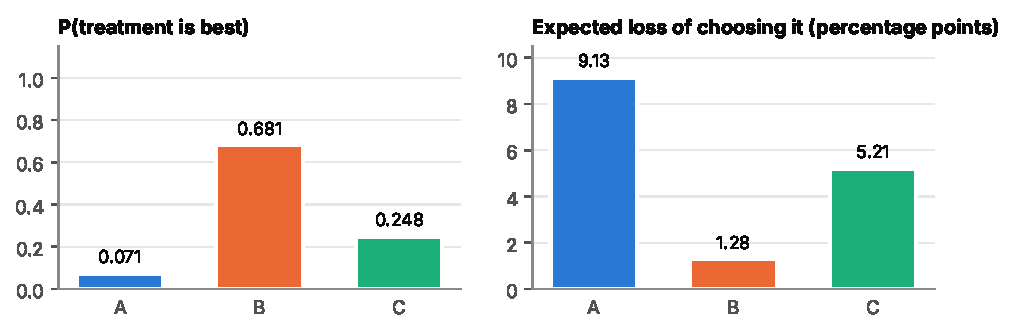
\includegraphics[width=0.86\linewidth]{fig3_best.pdf}
\caption{Left: posterior probability that each treatment is the best. Right: expected opportunity
loss of choosing each treatment, $E[\max_j\theta_j-\theta_k\mid\text{data}]$, in percentage points.}
\label{fig:best}
\end{figure}

\section{Recommendation (question 7)}

\textbf{Choosing a treatment is a Bayes decision.} The Bayes action minimises posterior expected loss
\course{Module~4, Definition~4.3, p.\,7}. Two natural losses give the same answer:
\begin{itemize}
\item \emph{Opportunity loss} $L(\boldsymbol\theta,k)=\max_j\theta_j-\theta_k$ is the success rate
given up by not choosing the best treatment. Its posterior expectation is
$E[\max_j\theta_j]-E[\theta_k]$, and $E[\max_j\theta_j]=\emax$ does not depend on $k$, so the Bayes
action is the largest posterior mean. The expected losses are $\elossptsB$ (B), $\elossptsC$ (C) and
$\elossptsA$ (A) percentage points.
\item \emph{Zero--one loss} (1 if the chosen treatment is not the best) has posterior expected loss
$1-P(k\text{ best})$, so the Bayes action is the treatment most likely to be best.
\end{itemize}
Both losses choose B, just as the squared-error and zero--one losses gave the posterior mean and mode
for a single $\theta$.

\begin{table}[H]
\centering\small
\caption{Prior sensitivity. The same priors are used for all three treatments.}\label{tab:sens}
\begin{tabular}{lcccccc}
\toprule
Prior & $E[\tB\mid\text{data}]$ & $P(\tB>\tA)$ & $P(\tB>\tC)$ & $P(\text{B best})$ & Exp.\ loss of B & Choice\\
\midrule
Uniform $\Beta(1,1)$ & $\sUnimeanB$ & $\sUnipBA$ & $\sUnipBC$ & $\sUnipbestB$ & $\sUnielossB$ & \sUnidec\\
Jeffreys $\Beta(\tfrac12,\tfrac12)$ & $\sJefmeanB$ & $\sJefpBA$ & $\sJefpBC$ & $\sJefpbestB$ & $\sJefelossB$ & \sJefdec\\
$\Beta(2,2)$ & $\sBttmeanB$ & $\sBttpBA$ & $\sBttpBC$ & $\sBttpbestB$ & $\sBttelossB$ & \sBttdec\\
$\Beta(10,10)$ & $\sBtenmeanB$ & $\sBtenpBA$ & $\sBtenpBC$ & $\sBtenpbestB$ & $\sBtenelossB$ & \sBtendec\\
\bottomrule
\end{tabular}
\end{table}

\textbf{Robustness to the prior.} Table~\ref{tab:sens} repeats the analysis with the Jeffreys prior
\course{Module~4, \S5.3.3, p.\,14} and the two priors of assignment problems 1.2 and 1.12. Even
$\Beta(10,10)$, which is worth 20 imaginary patients centred on 50\%, changes $P(\text{B best})$ only
from $\sUnipbestB$ to $\sBtenpbestB$. The choice is B every time, so the conclusion does not depend on
the prior.

\textbf{How strong is the evidence?} B is very probably better than A ($\pgtBA$). It is only modestly
likely to be better than C ($\pgtBC$), and its 95\% credible interval for $\tB-\tC$ runs from
$\dloBC$ to $\dhiBC$. Figure~\ref{fig:more} shows how this would change with more patients, under
the purely illustrative assumption that the success rates stayed exactly as observed. Then
$P(\text{B best})$ would first reach $0.95$ at about $\scencross$ patients per arm, seven and a half
times the present trial. This is not a prediction; real future data will vary.

\begin{figure}[H]
\centering
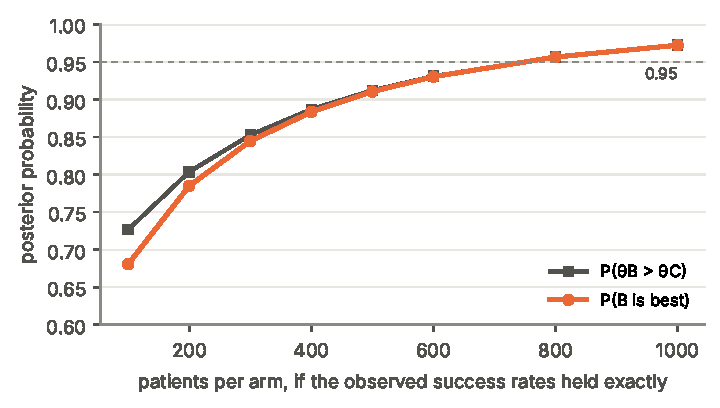
\includegraphics[width=0.62\linewidth]{fig4_more_data.pdf}
\caption{Posterior probabilities for B if each arm had more patients with the same observed success
rates (illustration only).}
\label{fig:more}
\end{figure}

\textbf{Recommendation.} \emph{Choose treatment B.} It has the highest estimated success rate
($\meanB$; 95\% CrI $\criloB$--$\crihiB$) and the highest probability of being best ($\pbestB$). It
also carries the smallest expected cost of being wrong: $\elossptsB$ percentage points of success
rate, against $\elossptsC$ for C and $\elossptsA$ for A. This holds under all four priors. Because B
and C are not clearly separated, a decision with serious consequences, or one where B is more
costly or has more side effects, would justify a further trial comparing B with C.

\section{Course method check: Lindley and Tierney--Kadane (Module 5)}

Module~5 approximates a posterior expectation $E[u(\theta)\mid\mathbf{x}]$ when it has no closed
form. Lindley's method \course{slides 7--11} expands around the MLE:
$E[u]\approx u(\hat\theta)+\tfrac12\sigma^2(u_2+2u_1\rho_1)+\tfrac12\sigma^4L_3u_1$, with
$\sigma^2=-1/L_2(\hat\theta)$. The Tierney--Kadane method \course{slides 13--19} uses
$E[u]\approx(\sigma_*/\sigma_0)\exp\{n[L_*(\hat\theta_*)-L_0(\hat\theta_0)]\}$. Our problem has exact
conjugate answers, so it measures their error directly: $E[\theta]=a/(a+b)$ and
$E[\theta/(1-\theta)]=a/(b-1)$ for a $\Beta(a,b)$ posterior. Before applying the methods, we checked
that our implementation reproduces the course's own worked example: Lindley $1.9965$ (slide~12) and
Tierney--Kadane $1.995138$ (slides 18--19).

\begin{table}[H]
\centering\small
\caption{Module 5 approximations against exact posterior expectations (uniform prior). Error =
approximation $-$ exact.}\label{tab:m5}
\begin{tabular}{lcccccc}
\toprule
 & \multicolumn{3}{c}{$E[\theta\mid\text{data}]$} & \multicolumn{3}{c}{$E[\theta/(1-\theta)\mid\text{data}]$ (odds)}\\
\cmidrule(lr){2-4}\cmidrule(lr){5-7}
 & Exact & Lindley error & T--K error & Exact & Lindley error & T--K error\\
\midrule
A & $\mmeanexA$ & $\mmeanlierrA$ & $\mmeantkerrA$ & $\moddsexA$ & $\moddslierrA$ & $\moddstkerrA$\\
B & $\mmeanexB$ & $\mmeanlierrB$ & $\mmeantkerrB$ & $\moddsexB$ & $\moddslierrB$ & $\moddstkerrB$\\
C & $\mmeanexC$ & $\mmeanlierrC$ & $\mmeantkerrC$ & $\moddsexC$ & $\moddslierrC$ & $\moddstkerrC$\\
\bottomrule
\end{tabular}
\end{table}

Both methods are accurate to about $10^{-4}$, the $O(n^{-2})$ order the slides predict for $n=100$.
For the posterior mean, Lindley simplifies to $s/n+(n-2s)/n^2$. For the odds, its three terms add up to
\[
\frac{s}{n-s}+\frac{s}{(n-s)^2}+\frac{n-2s}{(n-s)^2}=\frac{s+1}{n-s},
\]
which is exactly the conjugate answer, so its error in Table~\ref{tab:m5} is zero.

\section{Limitations}

\begin{itemize}
\item \textbf{Simulated data.} The figures come from the project sheet, not a real trial, and the
conclusions apply only to these numbers.
\item \textbf{Independence and a common rate.} The model assumes that patients within an arm are
independent with a common success probability, and that the arms are independent. Different patient
populations across arms, clustering (for example by hospital) or a non-randomised allocation would
break this.
\item \textbf{One outcome.} Success is the only outcome. Costs, side effects and severity of failure
are ignored, and any of them could change the decision.
\item \textbf{No pooling across treatments.} Independent priors treat the three rates as unrelated.
A hierarchical model would let them share information, but it is a multi-parameter model outside the
single-parameter course syllabus.
\end{itemize}

\section{Reproducibility and verification}

Every computed result in this report is written by \texttt{scripts/run\_analysis.py} into a file
that the report reads, so no result was copied by hand. The remaining figures in the text (the data,
the course's worked-example values and descriptive ranges such as ``$\pm9$ percentage points'') are
checked separately in \texttt{checks/test\_report.py}. Each exact result was verified by a second exact method
(the finite-sum formula, the binomial-tail form of the CDF, or a second integration order), by
quadrature and by seeded Monte Carlo judged by its standard error. The conjugate posterior was also
checked against Bayes' theorem evaluated numerically on a grid. The checks run with
\texttt{python checks/run\_checks.py}.

\appendix
\section{Course mapping}
\begin{table}[H]
\centering\small
\begin{tabular}{p{0.47\linewidth}p{0.47\linewidth}}
\toprule
Topic used & Course source\\
\midrule
Bernoulli and binomial distributions & Module 1, \S1.2--1.3, pp.\,5--9\\
Normal distribution, $\Phi$ (Wald intervals) & Module 1, \S2.5, pp.\,24--29; assignment 1.7--1.8\\
Independence of the three arms & Module 2, Definition 2.8, p.\,9\\
Sufficiency of $s$ (Neyman--Fisher factorisation) & Module 3, \S2, p.\,4\\
MLE $\hat\theta=s/n$ & Module 3, p.\,14\\
Beta--binomial conjugate posterior & Module 4, Examples 4.6, 4.9; \S5.1.1, pp.\,4--11\\
Posterior mean, median, mode as Bayes estimators & Module 4, Theorems 4.1--4.3, pp.\,7--8\\
Bayes action minimising posterior expected loss & Module 4, Definition 4.3, p.\,7\\
Jeffreys prior $\Beta(\tfrac12,\tfrac12)$ & Module 4, \S5.3.3, p.\,14\\
Lindley and Tierney--Kadane approximations & Module 5, slides 7--19\\
Simulation from the posterior, $P(\tB>\tA)$ & Module 5, slide 20; assignment 1.10\\
Credible intervals, prior sensitivity, predictive probability & Assignment problems 1.2, 1.11, 1.12\\
\bottomrule
\end{tabular}
\end{table}

\end{document}
